\documentclass[a4paper,12pt]{article}
\usepackage{fullpage}
\usepackage[utf8x]{inputenc}
\usepackage{fancyhdr}
\usepackage{booktabs}
\usepackage[hang,bf,small]{caption}
\usepackage{color}
\usepackage{graphicx}
\usepackage{multirow}
\usepackage{hyperref}
\usepackage{longtable}
\usepackage{subfig}


%set subfig package options
\captionsetup[subfloat]{position=top,singlelinecheck=false,labelfont={normalsize,sf},
labelformat=simple,listofformat=subparens,aboveskip=0pt,parskip=0pt,farskip=0pt,captionskip=0pt}

%customize subfigure label to capitals
\renewcommand{\thesubfigure}{\Alph{subfigure}}
\renewcommand{\thesubtable}{\textbf{\Alph{subtable}}}



\begin{document}

\begin{titlepage}

\begin{center}

\textsc{ }\\[2cm]
% Upper part of the page
%\includegraphics[width=0.7\textwidth]{img/logoTRANSPAT.jpg}\\[4cm]    


\textsc{\textcolor{blue}{\Huge \em Integrated Gene Set Analysis for microRNA Studies}}\\[2.5cm]

\textsc{\textcolor{blue}{\Large Comparison of methods for Gene Set Analysis}}\\[2.5cm]





%\includegraphics[width=0.3\textwidth]{img/logoERANET.jpg}\\[4cm]    


% Title
% \HRule \\[0.4cm]
% { \Large Computational Genomics Department}\\[0.4cm]
% { \Large CIPF, Valencia (Spain)}\\[0.4cm]



\vfill

% Bottom of the page
{\large \today}

\end{center}

\end{titlepage}


% \maketitle

\tableofcontents


% \begin{abstract}
% \end{abstract}
\cleardoublepage




\section{Methods}\label{secMethods}


A GSA extension of Godard’s approach have been  computed straight forward using logistic regression
models and our Bioconductor library. This strategy will certainly retain Godard’s methodology good
characteristics while incorporating the benefits of the GSA approach over the ORA one.

We did find that the functional results at miRNA level (Godard’s generalization) and the ones at gene level (after transference as originally proposed)
have a significantly positive correlation. This indicates that overall both methodologies should provide
similar findings. The correlation is not very strong though as the methodologies are explicitly different.

Detailed results and scripts are available in \url{https://github.com/dmontaner-papers/gsa4mirna}
(folders: supplementary\_files\_godard and scripts\_godard).


\clearpage



\section{Results}

For each cancer type, there are several plots displaying the correlation between the GSA analysis carried out at miRNA level (Godard’s paradigm)
 and at gene level after “transference”. Each dot represents a GO term. 
 X and Y values are derived from p-values and signs of the log odds ratios resulting from the mdgsa analysis
  (similar to equation 1 of the paper but at GO level instead of at miRNA level).

  
  
\begin{figure}[!h] 
\centering 
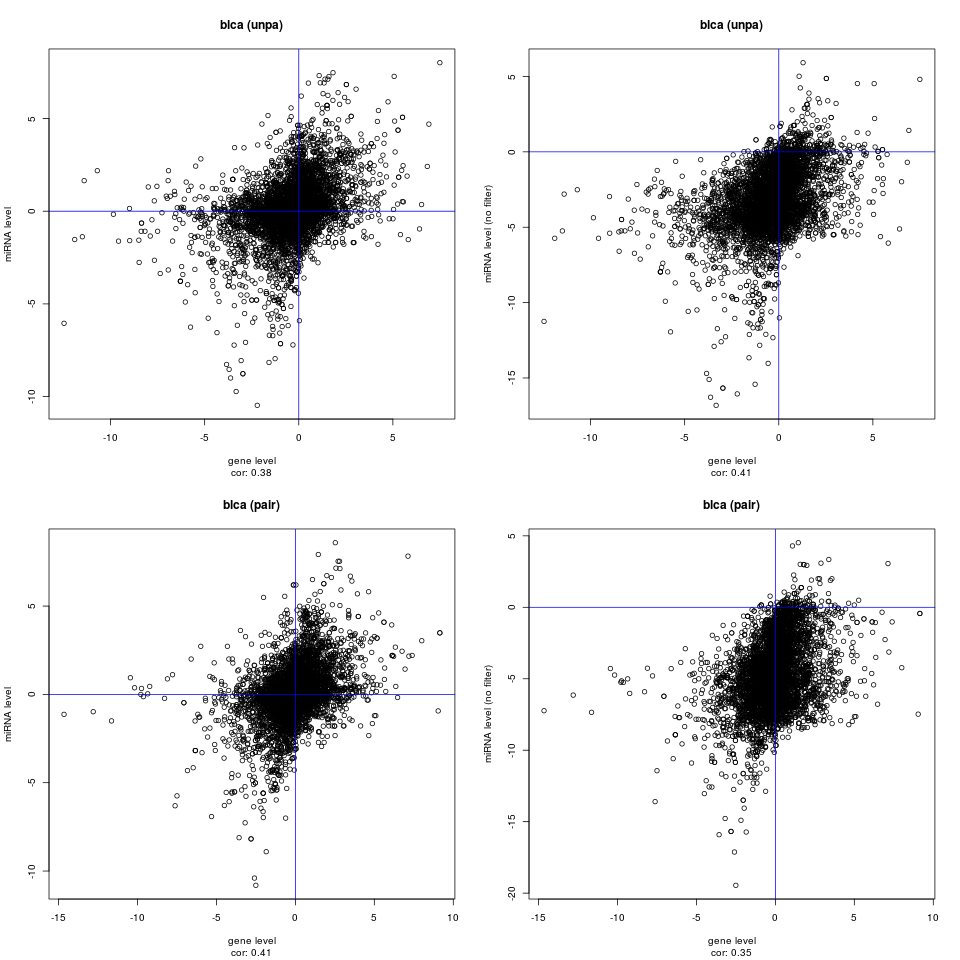
\includegraphics[width=0.9\textwidth]{plots/gene_vs_mirna_level_gsa_blca.png} 
\caption{BLCA} 
\end{figure} 

\newpage

\begin{figure}[!h] 
\centering 
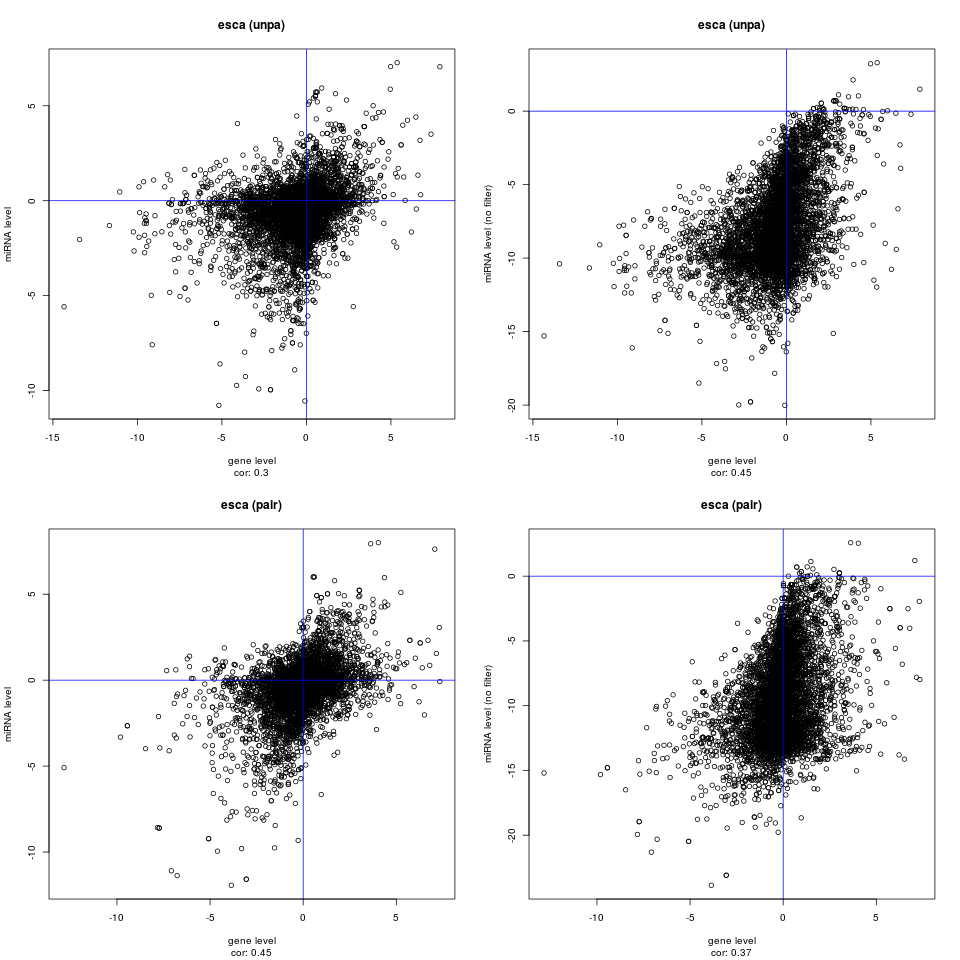
\includegraphics[width=0.9\textwidth]{plots/gene_vs_mirna_level_gsa_esca.png} 
\caption{ESCA} 
\end{figure} 

\newpage

\begin{figure}[!h] 
\centering 
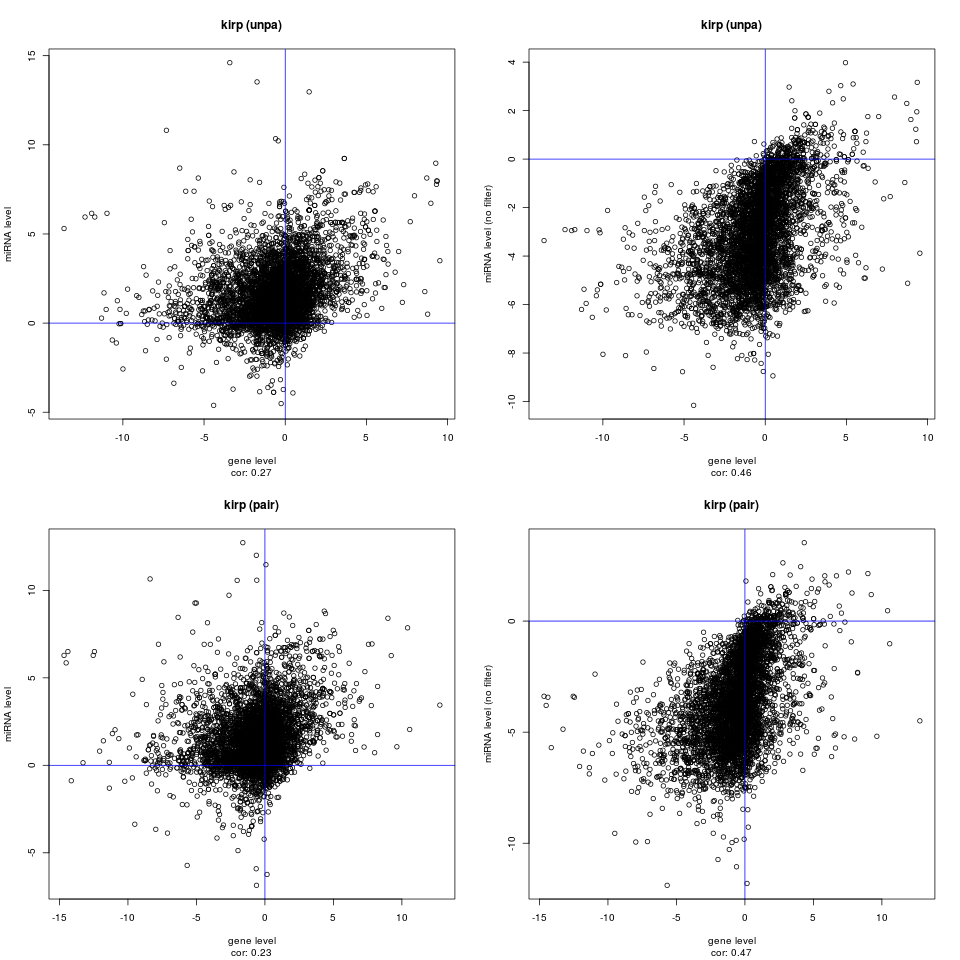
\includegraphics[width=0.9\textwidth]{plots/gene_vs_mirna_level_gsa_kirp.png} 
\caption{KIRP} 
\end{figure} 

\newpage

\begin{figure}[!h] 
\centering 
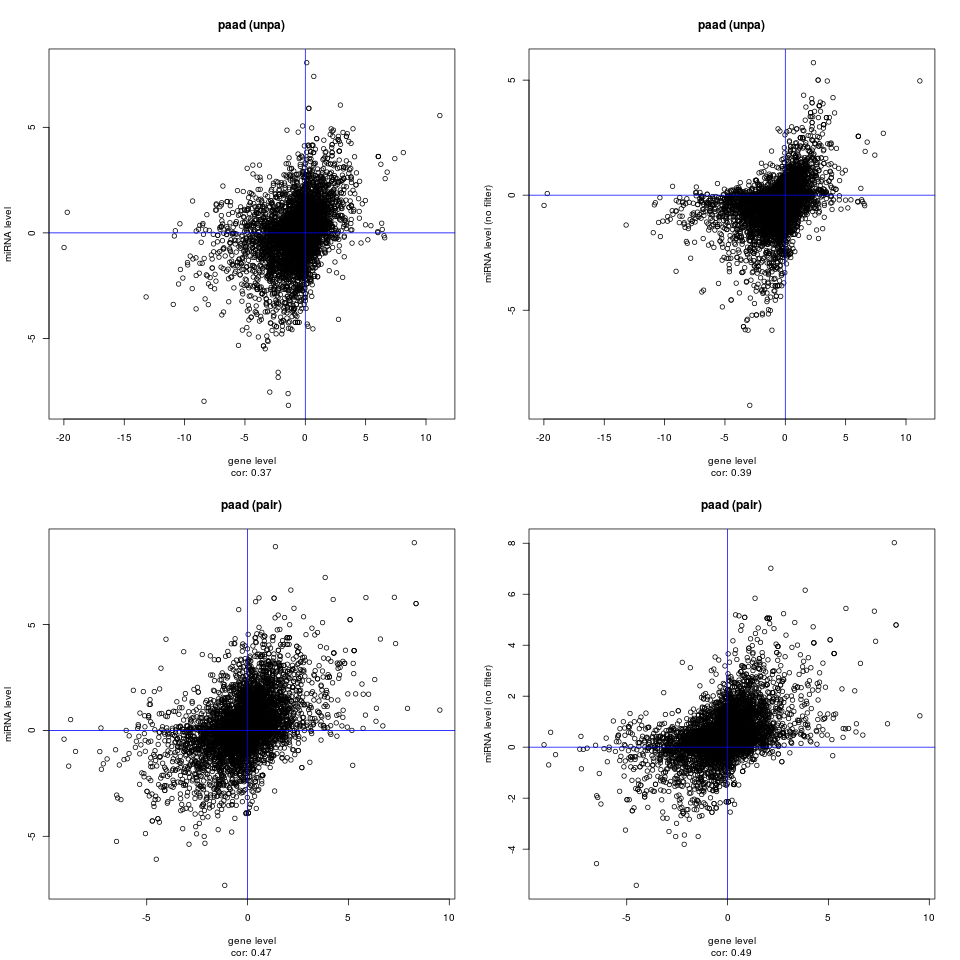
\includegraphics[width=0.9\textwidth]{plots/gene_vs_mirna_level_gsa_paad.png} 
\caption{PAAD} 
\end{figure} 

\newpage

\begin{figure}[!h] 
\centering 
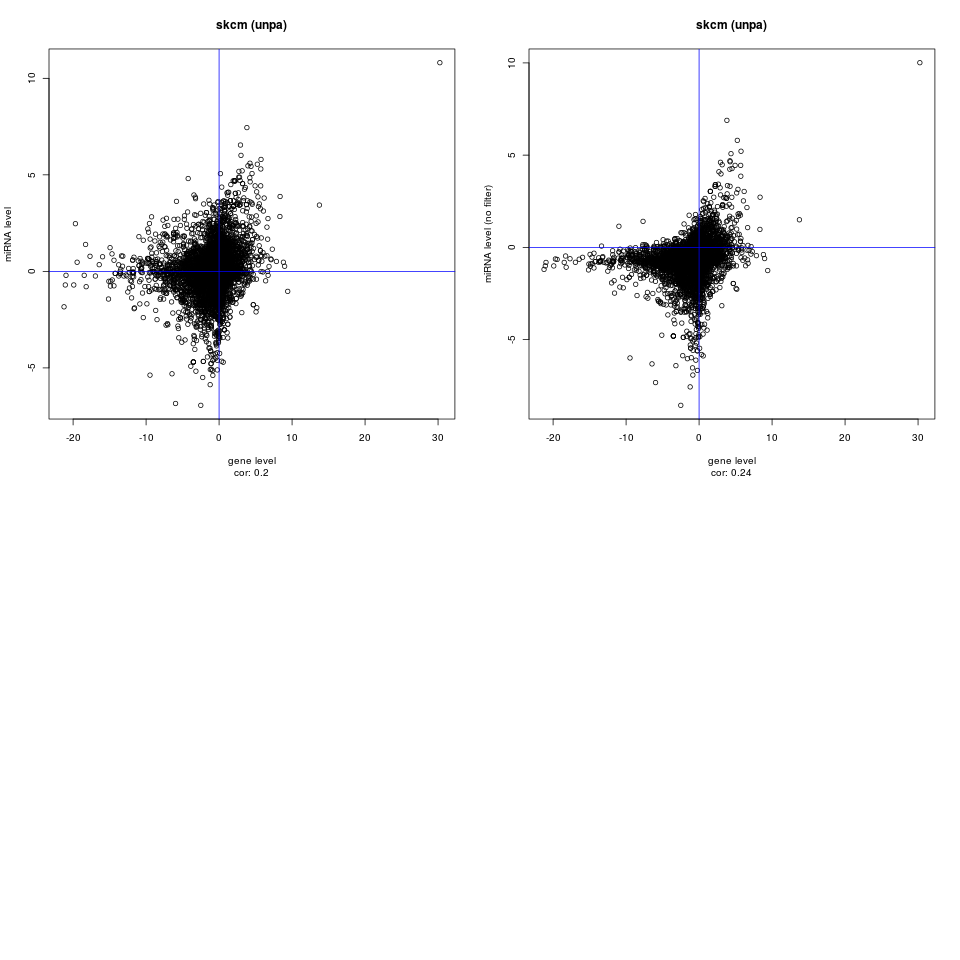
\includegraphics[width=0.9\textwidth]{plots/gene_vs_mirna_level_gsa_skcm.png} 
\caption{SKCM} 
\end{figure} 

\newpage

\begin{figure}[!h] 
\centering 
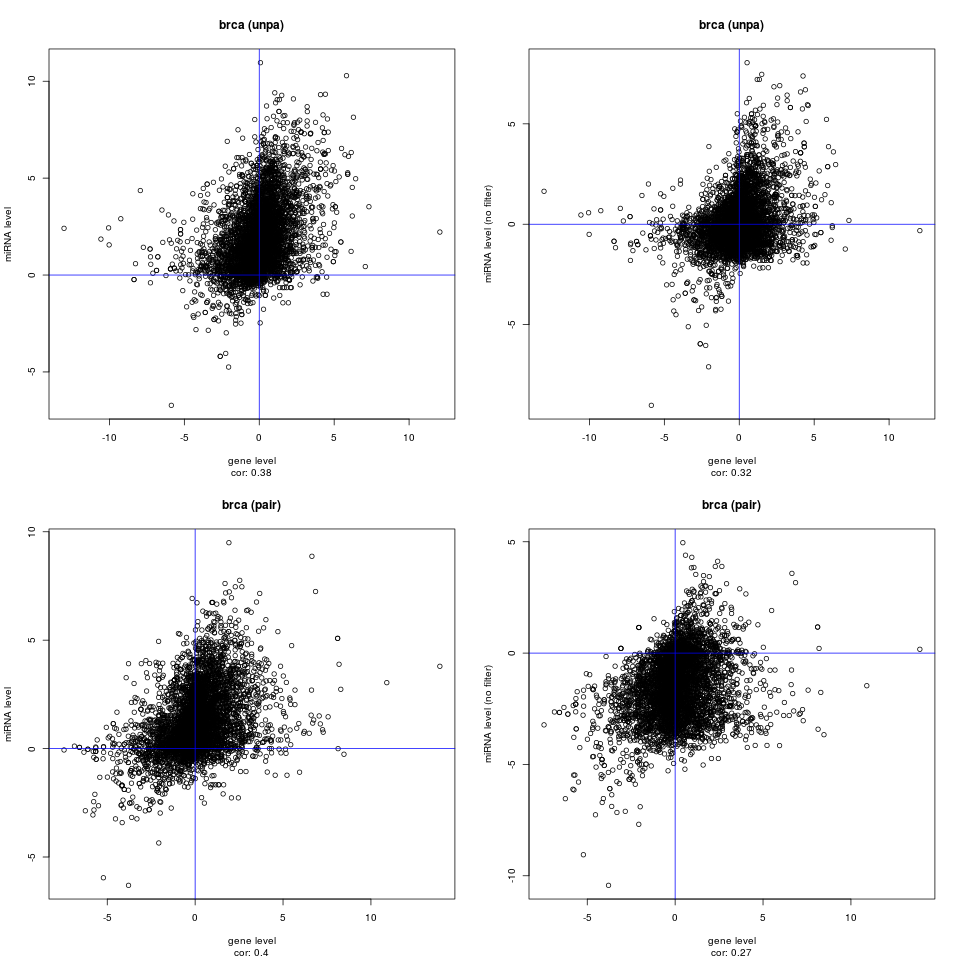
\includegraphics[width=0.9\textwidth]{plots/gene_vs_mirna_level_gsa_brca.png} 
\caption{BRCA} 
\end{figure} 

\newpage

\begin{figure}[!h] 
\centering 
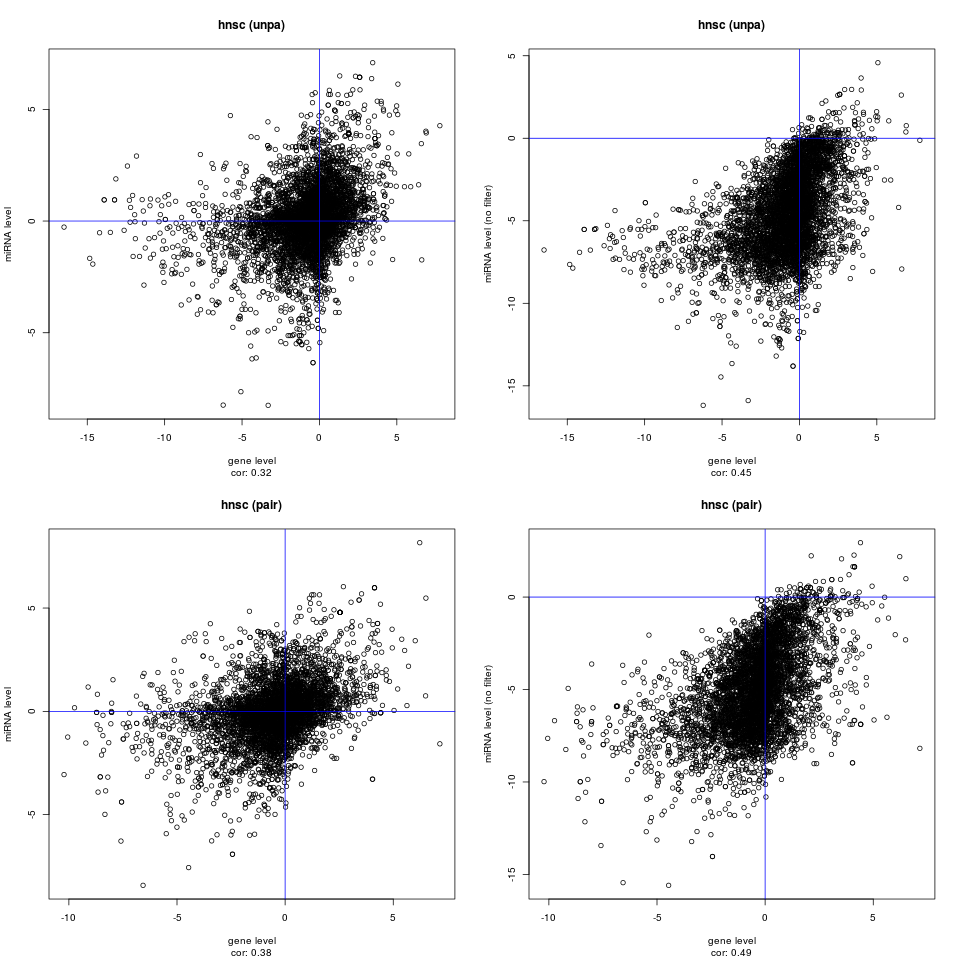
\includegraphics[width=0.9\textwidth]{plots/gene_vs_mirna_level_gsa_hnsc.png} 
\caption{HNSC} 
\end{figure} 

\newpage

\begin{figure}[!h] 
\centering 
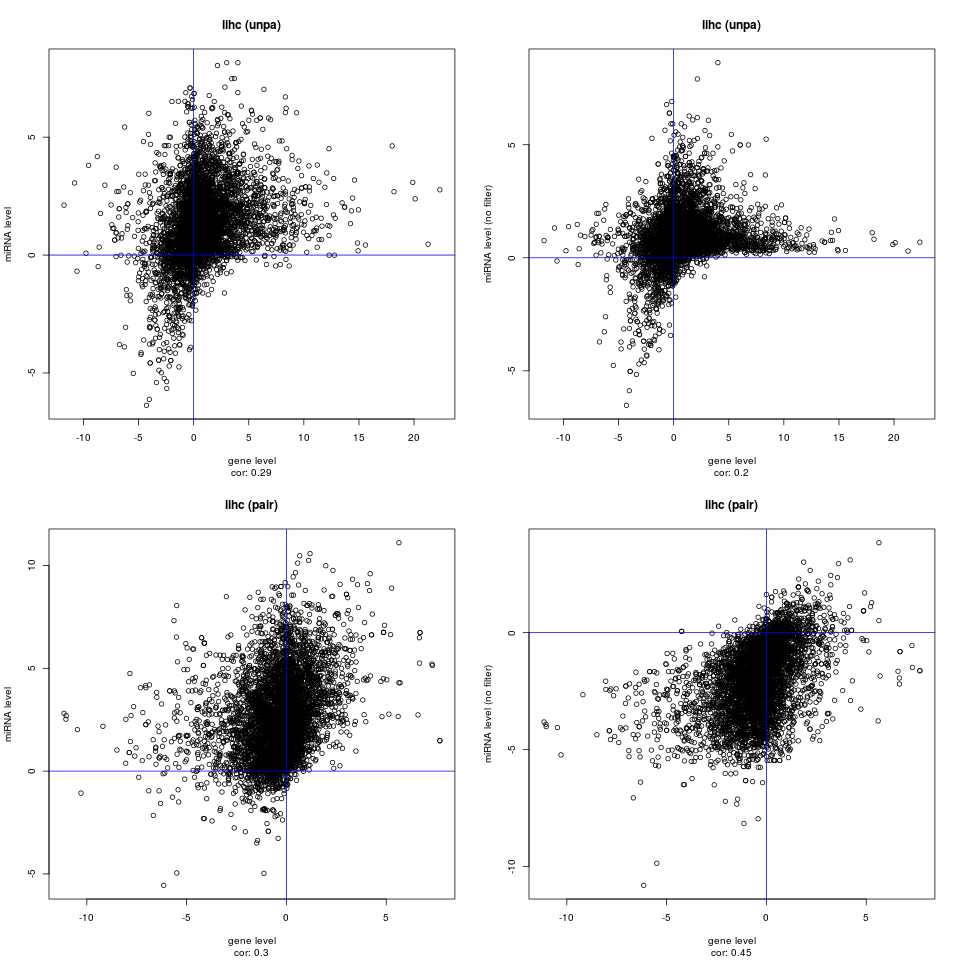
\includegraphics[width=0.9\textwidth]{plots/gene_vs_mirna_level_gsa_lihc.png} 
\caption{LIHC} 
\end{figure} 

\newpage

\begin{figure}[!h] 
\centering 
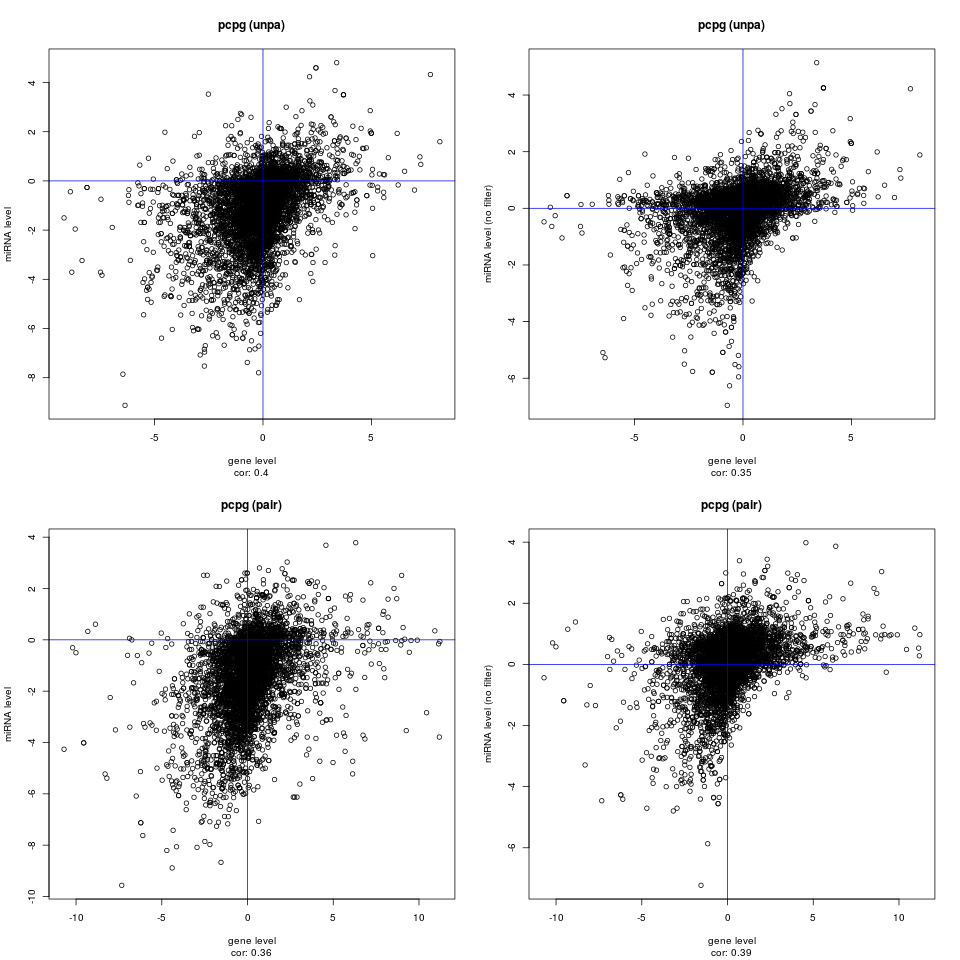
\includegraphics[width=0.9\textwidth]{plots/gene_vs_mirna_level_gsa_pcpg.png} 
\caption{PCPG} 
\end{figure} 

\newpage

\begin{figure}[!h] 
\centering 
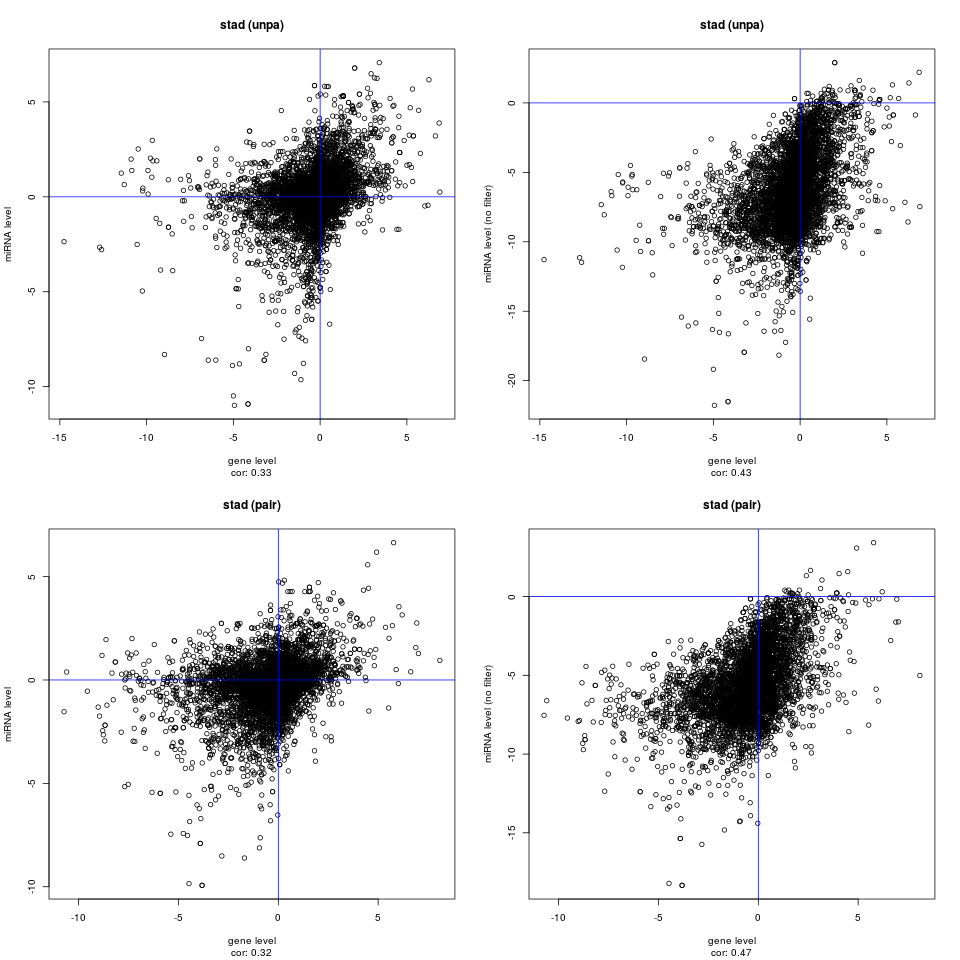
\includegraphics[width=0.9\textwidth]{plots/gene_vs_mirna_level_gsa_stad.png} 
\caption{STAD} 
\end{figure} 

\newpage




\begin{figure}[!h] 
\centering 
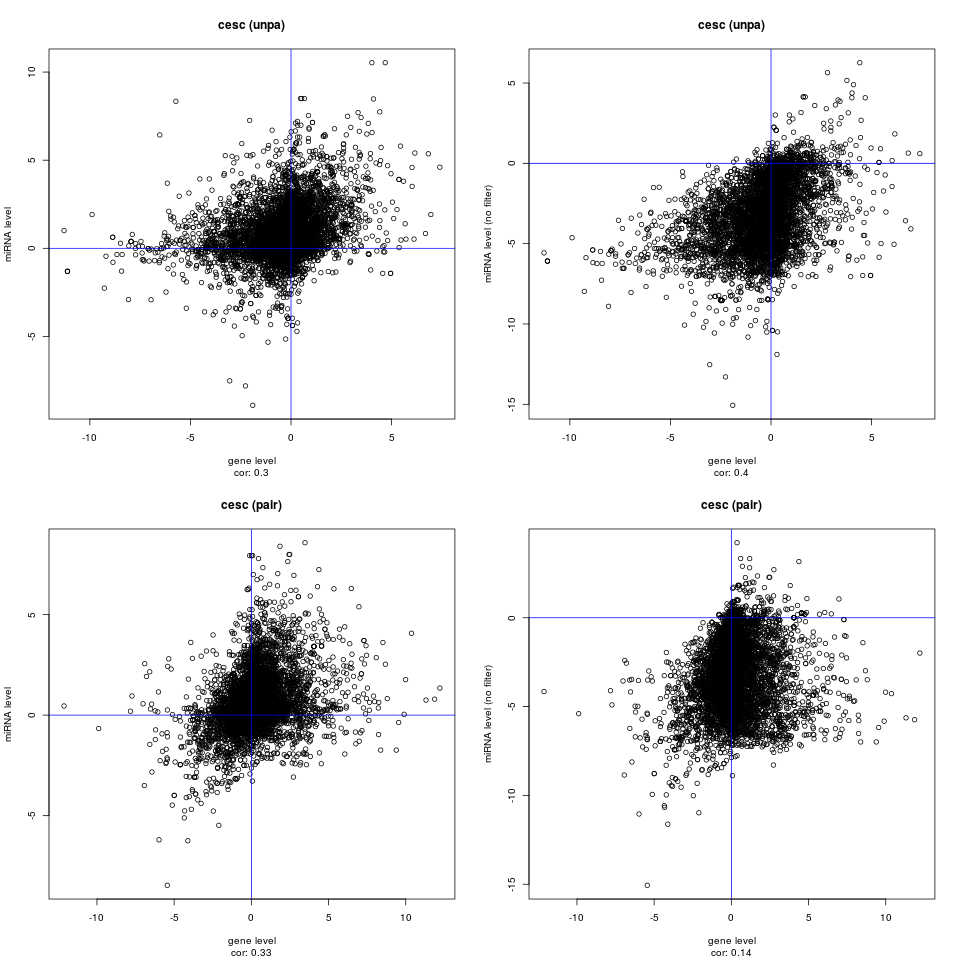
\includegraphics[width=0.9\textwidth]{plots/gene_vs_mirna_level_gsa_cesc.png} 
\caption{CESC} 
\end{figure} 

\newpage

\begin{figure}[!h] 
\centering 
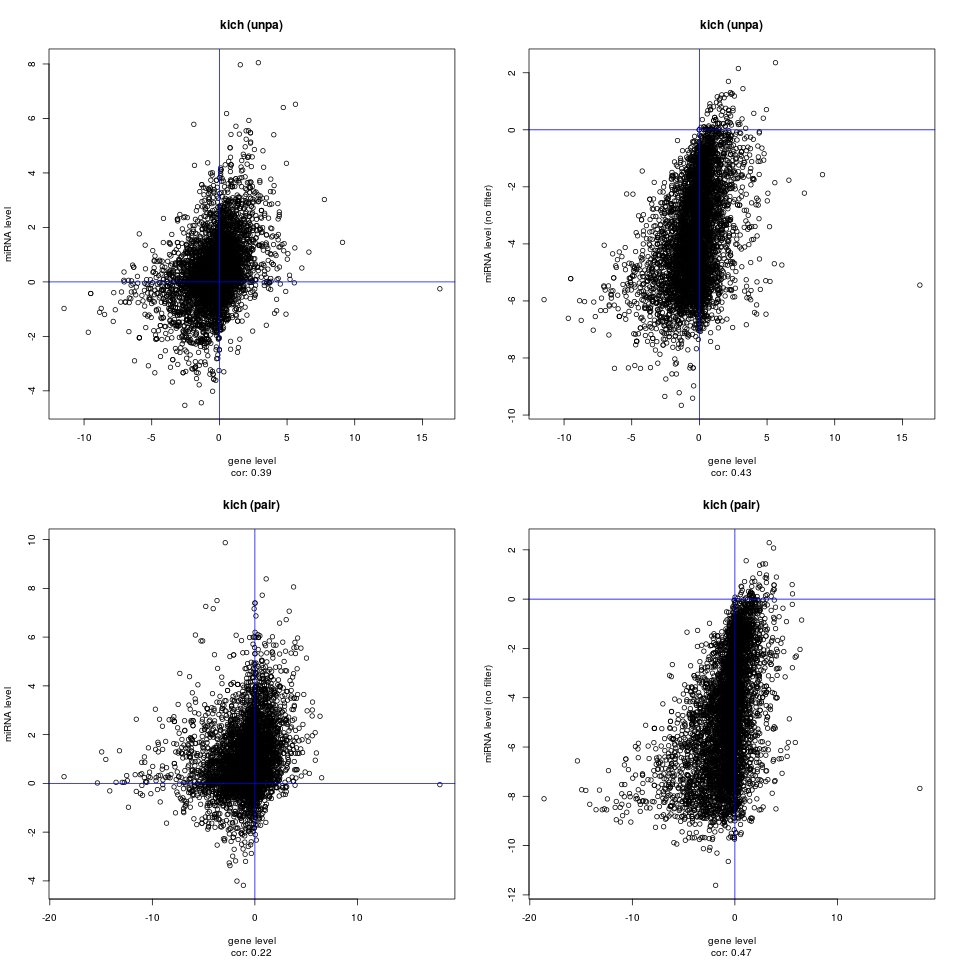
\includegraphics[width=0.9\textwidth]{plots/gene_vs_mirna_level_gsa_kich.png} 
\caption{KICH} 
\end{figure} 

\newpage

\begin{figure}[!h] 
\centering 
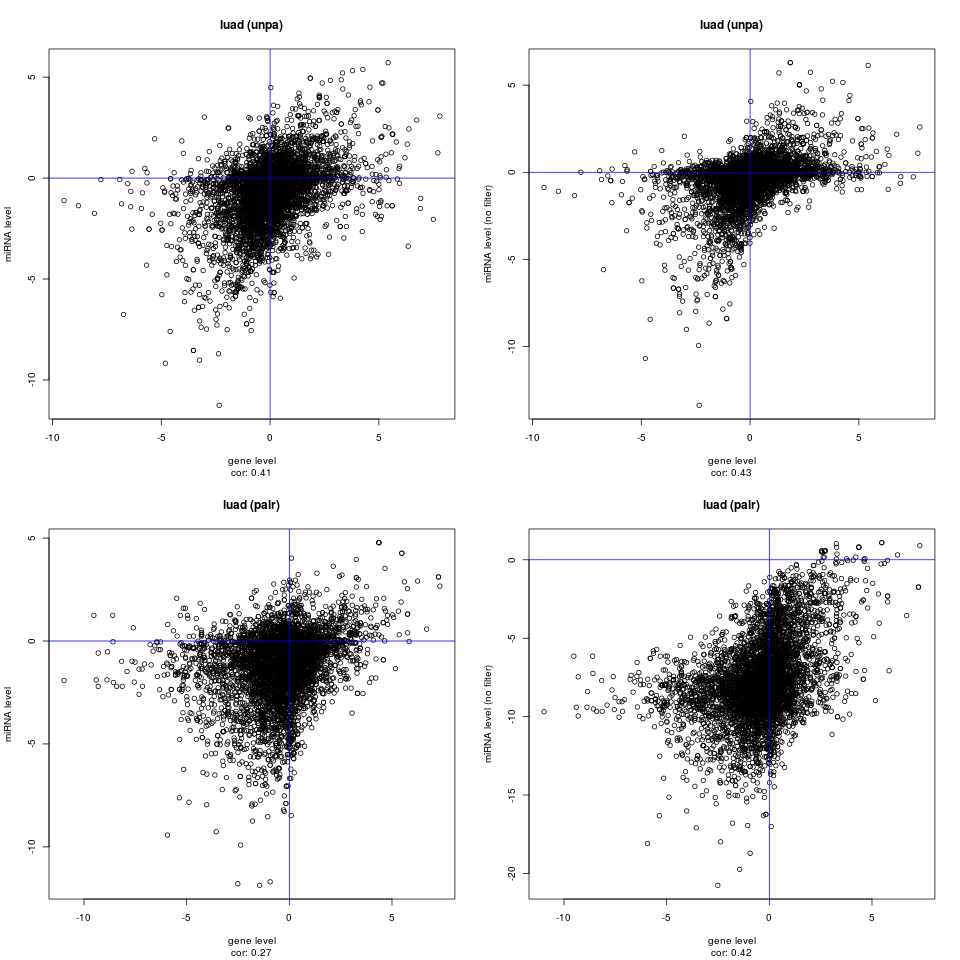
\includegraphics[width=0.9\textwidth]{plots/gene_vs_mirna_level_gsa_luad.png} 
\caption{LUAD} 
\end{figure} 

\newpage

\begin{figure}[!h] 
\centering 
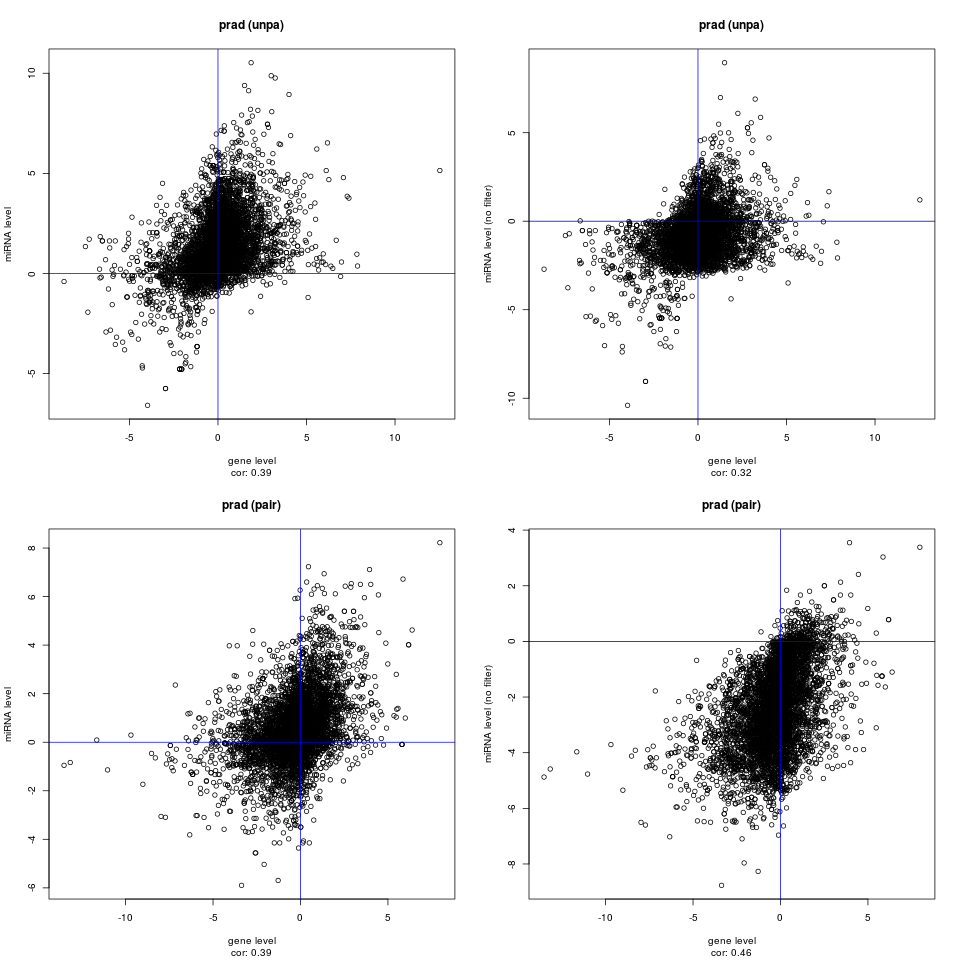
\includegraphics[width=0.9\textwidth]{plots/gene_vs_mirna_level_gsa_prad.png} 
\caption{PRAD} 
\end{figure} 

\newpage

\begin{figure}[!h] 
\centering 
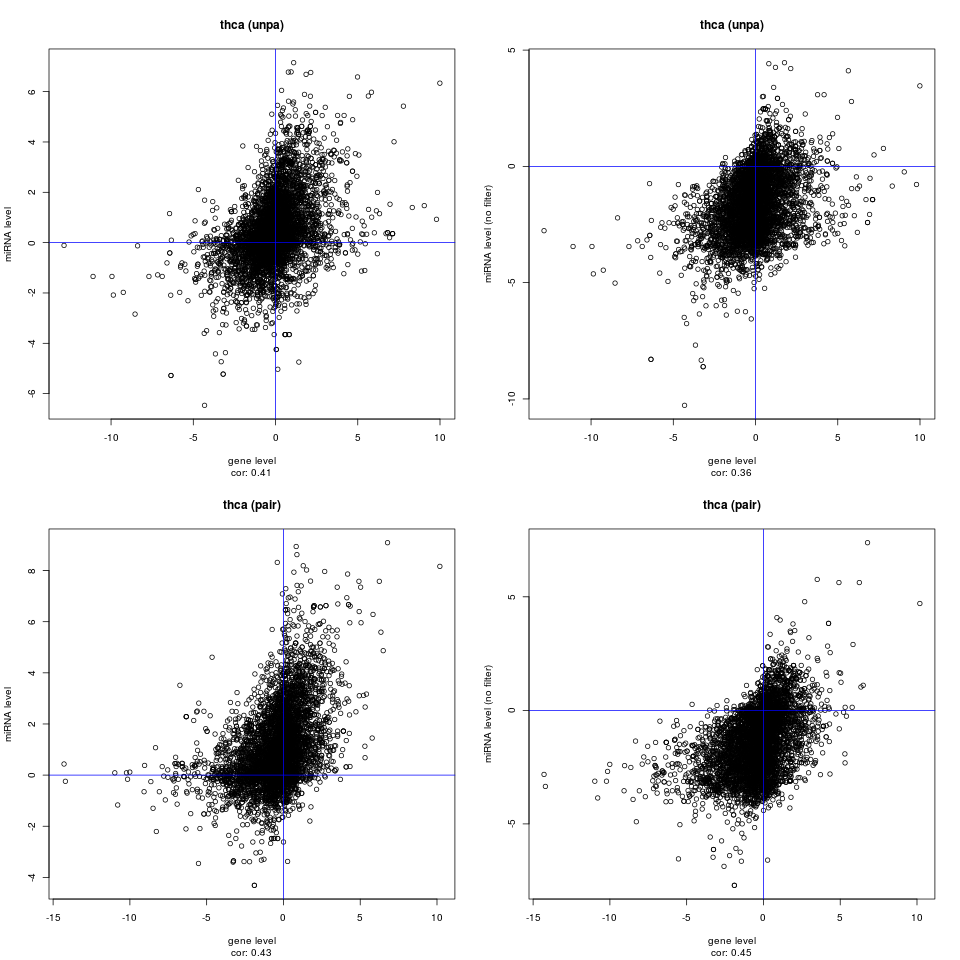
\includegraphics[width=0.9\textwidth]{plots/gene_vs_mirna_level_gsa_thca.png} 
\caption{THCA} 
\end{figure} 

\newpage

\begin{figure}[!h] 
\centering 
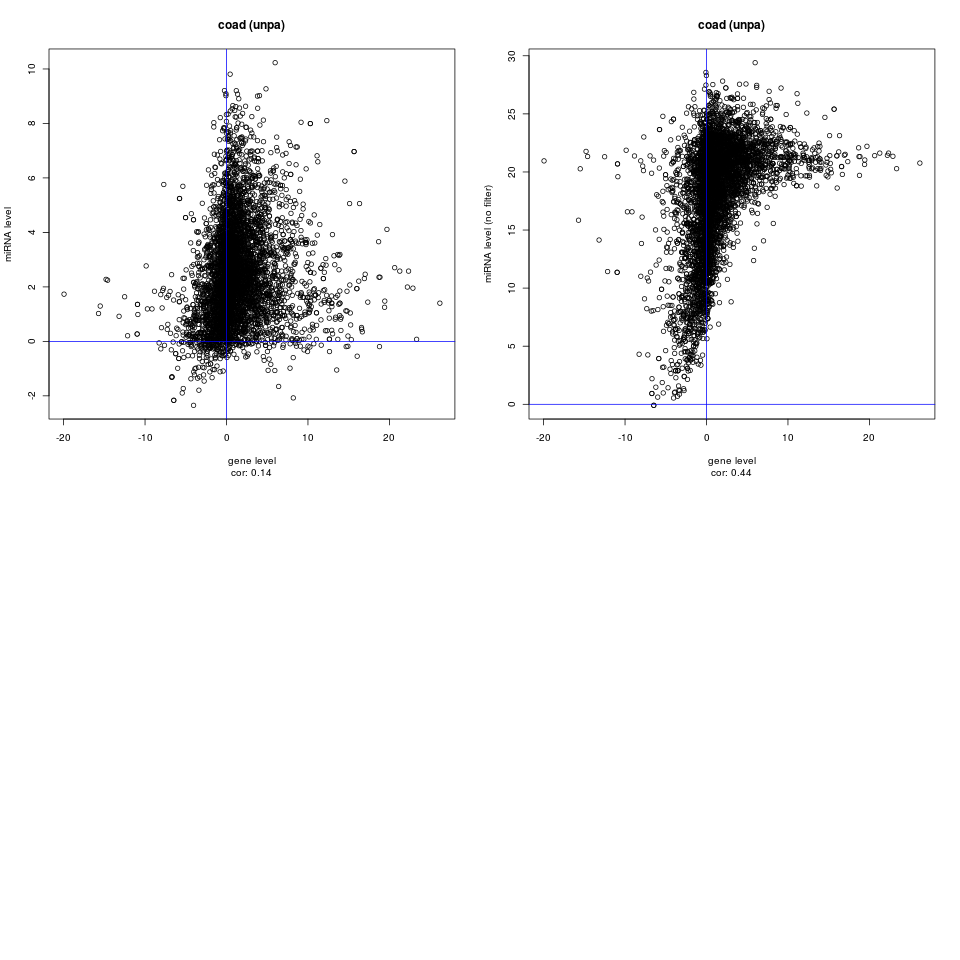
\includegraphics[width=0.9\textwidth]{plots/gene_vs_mirna_level_gsa_coad.png} 
\caption{COAD} 
\end{figure} 

\newpage

\begin{figure}[!h] 
\centering 
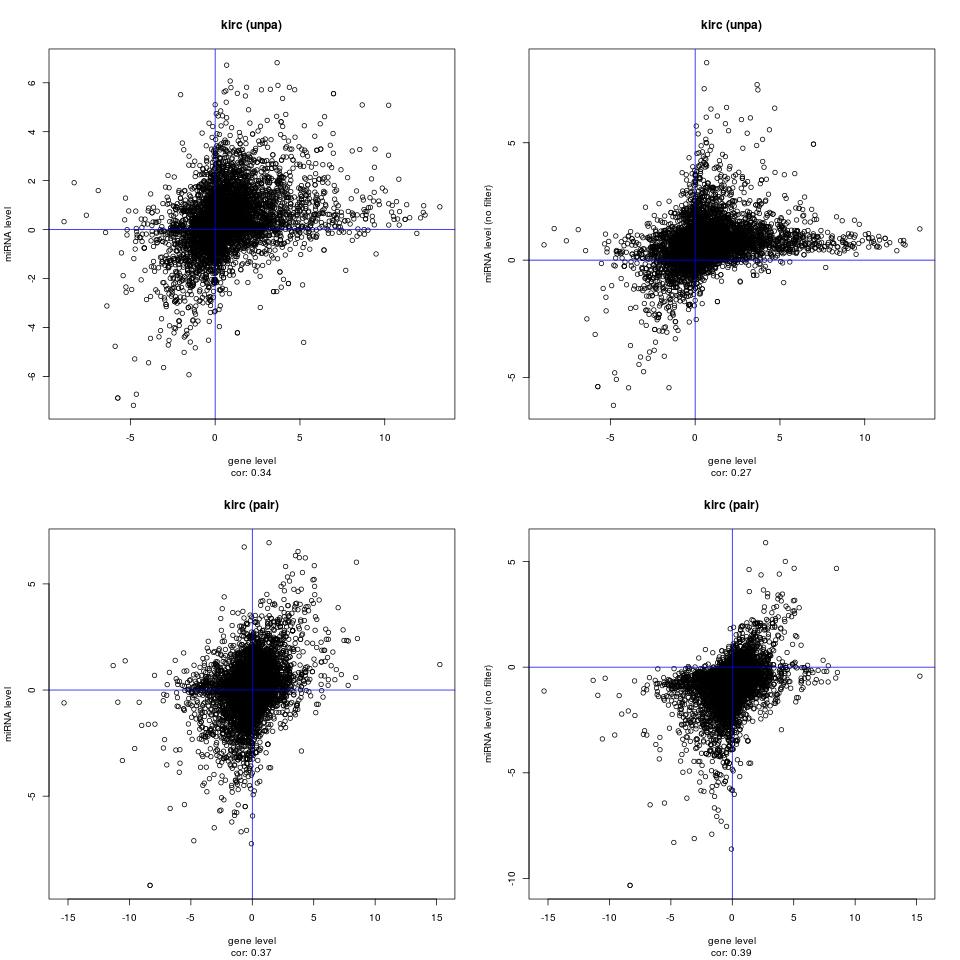
\includegraphics[width=0.9\textwidth]{plots/gene_vs_mirna_level_gsa_kirc.png} 
\caption{KIRC} 
\end{figure} 

\newpage

\begin{figure}[!h] 
\centering 
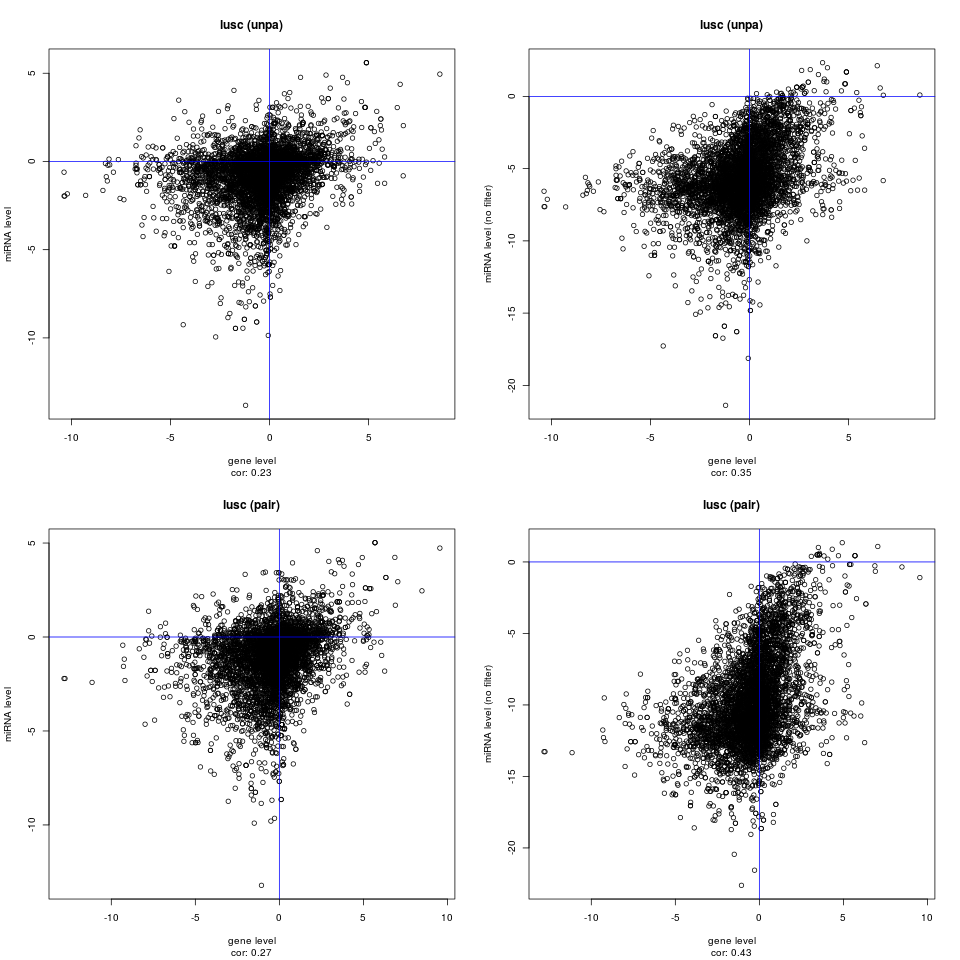
\includegraphics[width=0.9\textwidth]{plots/gene_vs_mirna_level_gsa_lusc.png} 
\caption{LUSC} 
\end{figure} 

\newpage

\begin{figure}[!h] 
\centering 
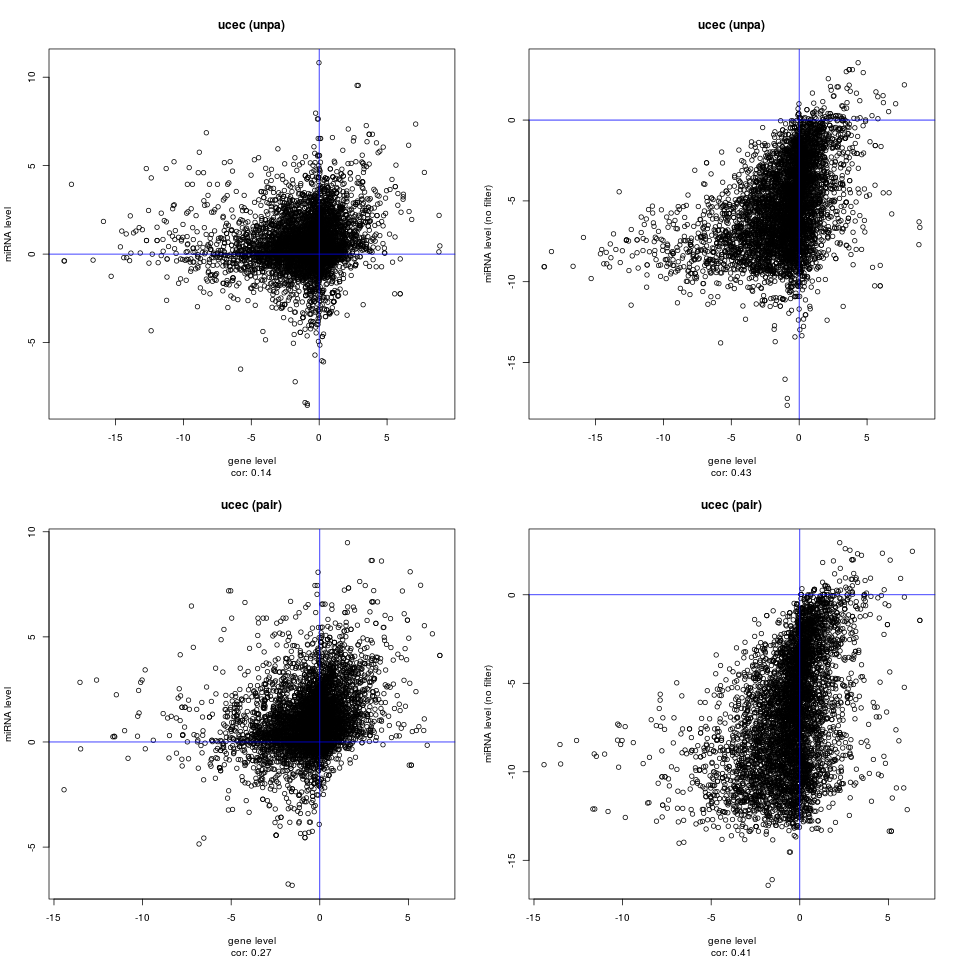
\includegraphics[width=0.9\textwidth]{plots/gene_vs_mirna_level_gsa_ucec.png} 
\caption{UCEC} 
\end{figure} 

\newpage

\begin{figure}[!h] 
\centering 
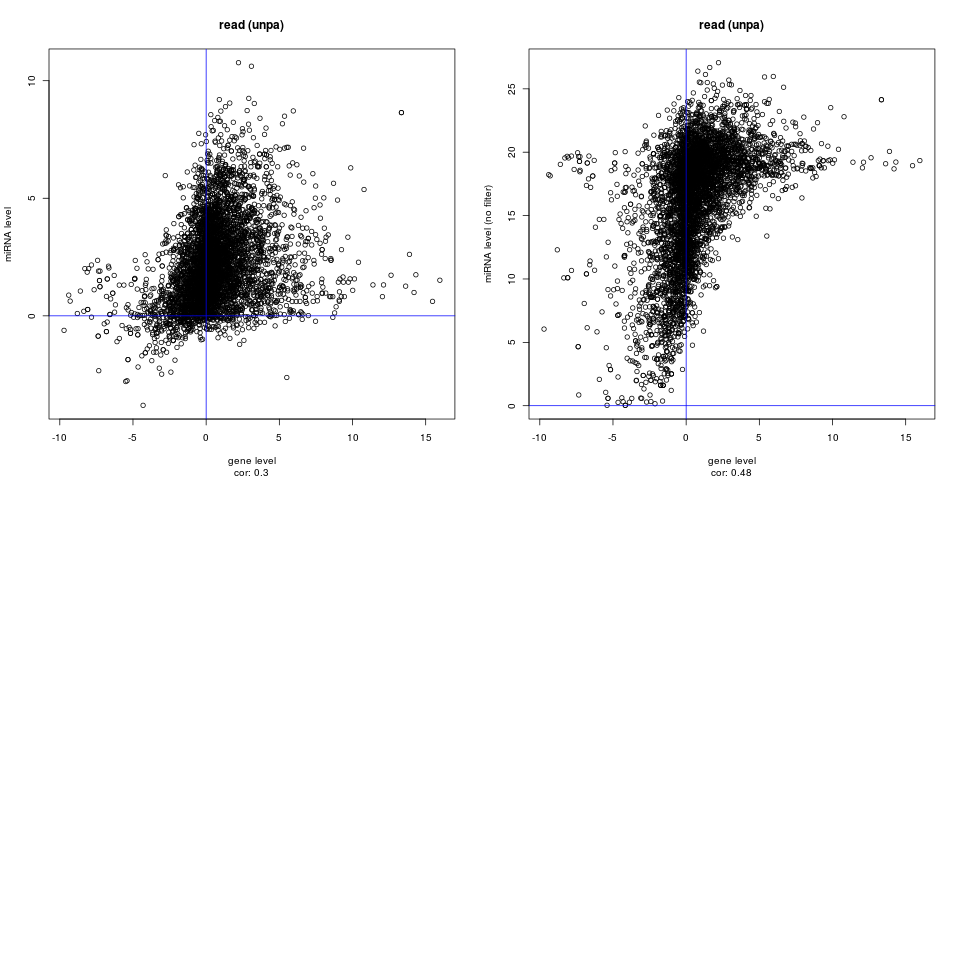
\includegraphics[width=0.9\textwidth]{plots/gene_vs_mirna_level_gsa_read.png} 
\caption{READ} 
\end{figure} 



\clearpage








% \addcontentsline{toc}{section}{References}
% % \addcontentsline{toc}{chapter}{\numberline{}\bibname}
% 
% 
% \bibliographystyle{abbrv}
% \bibliography{clustering}
% \begin{itemize}
%  \item Everitt, B. (1974). Cluster Analysis. London: Heinemann Educ. Books.
%  \item Suzuki R and Shimodaira H (2006).  Pvclust: an R package for assessing the uncertainty in hierarchical clustering. Bioinformatics. Jun 15;22(12):1540-2. Epub 2006 Apr 4.
%  \item Montaner D and Dopazo J (2010). Multidimensional Gene Set Analysis of Genomic Data. PLoS One, 5(4), pp. e10348. 
% \end{itemize}







\end{document}   
